\documentclass[presentation]{beamer}
\usepackage{newcent}
\usepackage[utf8]{inputenc}
\usepackage[T1]{fontenc}
\usepackage[czech]{babel}
\usepackage{hyperref}
\usepackage{graphicx}
\usepackage{caption}
\usepackage{subcaption}
\usetheme{FIT}

\date{10. 6. 2019}
\title[PWA v Haskellu]{Nástroj pro tvorbu Progressive Web Applications v Haskellu}
\author[]{Jakub Zárybnický}
\institute[]{Brno University of Technology, Faculty of Information Technology\\
Božetěchova 1/2. 612 66 Brno-Královo Pole\\
xzaryb00@stud.fit.vutbr.cz}

\begin{document}

\frame[plain]{\titlepage}

\begin{frame}{Úvod}
  \begin{itemize}
    \item Haskell v prohlížeči
    \item Interaktivní, offline, přístupné aplikace
    \item Open-source knihovny pro komunitu
  \end{itemize}
\end{frame}

\begin{frame}{Motivace}
  \begin{itemize}
    \item Funkcionální jazyky v prohlížeči
      \medskip
    \item Časté dotazy v komunitě Haskellu
    \item Základy jsou k dispozici, mnoho ale chybí
      \medskip
    \item PWA = technologie pro přístupnější webové aplikace
  \end{itemize}
\end{frame}

\begin{frame}{Náplň}
  \begin{itemize}
    \item Rešerže
      \begin{itemize}
        \item moderní webové frameworky
        \item knihovny chybějící v Haskellu
      \end{itemize}\medskip
    \item Knihovny
      \begin{itemize}
        \item Router (směrovač)
        \item Úložiště klíč-hodnota
        \item Service Worker
        \item Web Application Manifest
      \end{itemize}\medskip
    \item Aplikace
      \begin{itemize}
        \item TodoMVC
        \item HNPWA
        \item RealWorld
      \end{itemize}
  \end{itemize}
\end{frame}

\begin{frame}{Knihovny}
  \begin{figure}
    \centering
    \begin{minipage}{.5\textwidth}
      \centering
      
\includegraphics[width=.9\linewidth]{../doc-final-thesis/obrazky-figures/placeholder.pdf}
      \captionof{figure}{Router}
    \end{minipage}%
    \begin{minipage}{.5\textwidth}
      \centering
      
\includegraphics[width=.9\linewidth]{../doc-final-thesis/obrazky-figures/placeholder.pdf}
      \captionof{figure}{Storage}
    \end{minipage}
  \end{figure}

  \begin{figure}
    \centering
    \begin{minipage}{.5\textwidth}
      \centering
      
\includegraphics[width=.9\linewidth]{../doc-final-thesis/obrazky-figures/placeholder.pdf}
      \captionof{figure}{Service Worker}
    \end{minipage}%
    \begin{minipage}{.5\textwidth}
      \centering
      
\includegraphics[width=.9\linewidth]{../doc-final-thesis/obrazky-figures/placeholder.pdf}
      \captionof{figure}{WebManifest}
    \end{minipage}
  \end{figure}
\end{frame}

\begin{frame}{Aplikace}
  \begin{figure}
    \centering
    
\includegraphics[width=.45\linewidth]{../doc-final-thesis/obrazky-figures/screenshot-todomvc.png}
    \captionof{figure}{TodoMVC}
  \end{figure}

  \begin{figure}
    \centering
    \begin{minipage}{.5\textwidth}
      \centering
      
\includegraphics[width=.9\linewidth]{../doc-final-thesis/obrazky-figures/screenshot-hnpwa.png}
      \captionof{figure}{HNPWA}
    \end{minipage}%
    \begin{minipage}{.5\textwidth}
      \centering
      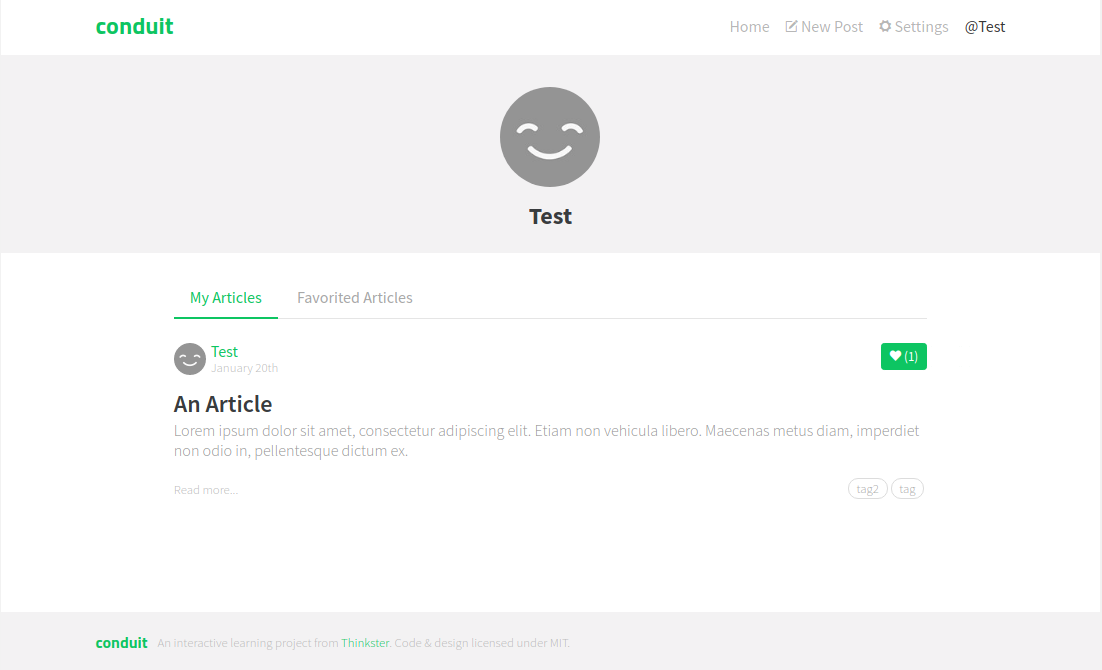
\includegraphics[width=.9\linewidth]{../doc-final-thesis/obrazky-figures/screenshot-realworld.png}
      \captionof{figure}{RealWorld}
    \end{minipage}
  \end{figure}
\end{frame}

\begin{frame}{Další kroky}
  \begin{itemize}
    \item Publikace knihoven
    \item Tvorba aplikací, které mě do této oblasti přivedly
    \item ...práce dle odezvy komunity
  \end{itemize}
\end{frame}

\bluepage{Děkuji za pozornost.}

\appendix
\begin{frame}{Otázky oponenta}
  \emph{Co je třeba dodělat, aby práce mohla být zveřejněna v archivu Hackage?}
  \medskip
  \begin{enumerate}
    \item Nutné pro publikování
      \begin{itemize}
        \item Hackage účet
        \item Licence
      \end{itemize}
    \item Očekávané od kvalitních balíčků
      \begin{itemize}
        \item Úplná dokumentace
        \item Ukázky použití
        \item Sada testů
        \item Continuous Integration
      \end{itemize}
  \end{enumerate}
\end{frame}

\end{document}

%%% Local Variables:
%%% mode: latex
%%% TeX-master: t
%%% End:
